\documentclass[../../../main.tex]{subfiles}
\begin{document}
Les pointeurs sont souvent considérés comme la source de bugs la plus fréquente en C. Cela résulte en général d'une mauvaise compréhension de leur manipulation et de manques de rigueur dans les codes utilisant les pointeurs.
Ce chapitre espère être suffisamment précis pour éviter au mieux les écueils habituels de la programmation avec des pointeurs\dots mais il n'est absolument pas certain que cela soit réussi.
 
\textbf{Rappel :} Une variable peut être approximée comme la collection de trois informations :
\begin{itemize}
	\item une étiquette, aussi appelée le nom de de la variable
	\item une adresse mémoire
	\item une donnée sur $N$ octets à cette adresse
\end{itemize}
Visuellement : 

\begin{minipage}{\textwidth}
	\begin{center}
		\includesvg[width=.25\textwidth]{variable}
	\end{center}
\end{minipage} 

L'idée des pointeurs est simple : au lieu de stocker directement une valeur, on stocke l'adresse mémoire d'une autre variable :

\begin{minipage}{\textwidth}
	\begin{center}
		\includesvg[width=.4\textwidth]{pointeur}
	\end{center}
\end{minipage}
 
Les pointeurs sont fondamentaux en C\footnote{Et presque seulement en C\dots}. En particulier, ils permettent une flexibilité très importante des programmes écrits. Ainsi, une variable d'une routine est locale à cette routine, et n'existe pas en dehors. Pourtant, une adresse mémoire peut potentiellement être utilisée hors de routines spécifiques, et l'utilisation de pointeurs permet de manipuler des variables bien qu'étant hors de l'environnement local de cette variable.

L'utilisation des pointeurs pour manipuler des adresses non locales décuple les possibilités des routines puisque celles-ci peuvent interagir avec leur environnement autrement que par la valeur de retour (dans le cas d'une fonction). Cela donne également une plus grande importance aux procédures.

% Cela amène cependant un inconvénient : en perdant un contrôle absolu sur l'existence de données, il devient possible \textit{par erreur} d'accéder à des zones mémoires qui ne sont plus utilisés. Il s'agit là de l'erreur la plus classique en programmation en C\footnote{traduite par le fameux message d'erreur \textit{Segmentation Fault}}.
 
Un pointeur est définit selon la syntaxe suivante :
\begin{minted}[linenos=false]{c}
TYPE* ptr;
\end{minted}
On sait alors que $ptr$ contiendra l'adresse d'une variable de type \textsf{TYPE} et va alors \textit{référer} à cette variable.

\subsection{Pointeurs et références}

On dispose pour la manipulation des pointeurs de deux opérateurs en langage C : l'étoile $\ast$ et l'esperluette $\&$.

L'esperluette en tant qu'opérateur binaire permet de signifier l'opération $ET$, qu'elle soit logique ou bit-à-bit. Comme opérateur unaire, \textit{$\&$v} renvoie l'adresse mémoire à laquelle se situe la variable \textit{v}. 

L'étoile en tant qu'opérateur binaire permet de signifier la multiplication numérique. Comme opérateur unaire, \textit{$^*$ptr} est une référence de la variable pointée par \textit{ptr}. Il s'agit d'accéder à la case mémoire contenue à une certaine adresse.

\begin{minipage}{\textwidth}
	\begin{center}
		\includesvg[width=0.5\textwidth]{indirection}
	\end{center}
\end{minipage}

On peut donc écrire :
\begin{minted}[linenos=false]{c}
double v = ...;
double* ptr = &v; // référence 'v' dans 'ptr'

// %p est le caractère de formatage d'une adresse mémoire :
printf("Adresse de v = %p = %p\n", &v, ptr);
printf("Valeur de v = %lf = %lf\n", v, *ptr);
\end{minted}
Ainsi :
\begin{itemize}
	\item $\&$ est l'opérateur de \textit{référencement} qui permet de contruire la référence d'une variable
	\item $^*$ est l'opérateur de \textit{déréférencement}\footnote{Ou d'indirection} qui permet d'accéder effectivement à la référence de la variable pointé
\end{itemize}
Le référencement permet de modifier la variable indirectement, \textit{via} le pointeur :
\begin{minted}[linenos=false]{c}
int v = 42; // déclaration et initialisation d'une variable
int* ptr = &v; // construire d'une "référence" vers 'v', &v est l'adresse de v
*ptr = 1001; // <=> v = 1001 par déréférencement de ptr
\end{minted}
On remarquera que $ptr$ doit être un pointeur de même type que le type de $v$. En effet, il devient possible depuis le pointeur $ptr$ de lire et de modifier la valeur de $v$. La pleine connaissance de $v$ est donc nécessaire, et l'information de son type est stockée comme le type du pointeur.

On peut décider également qu'un pointeur ne pointe sur rien grâce à la constante $\textsf{NULL} = 0$ :
\begin{minted}[linenos=false]{c}
int *pointeur = NULL; // ne pointe sur rien
\end{minted}
\textbf{Remarque/Avertissement :} Lorsqu'un pointeur ne pointe sur rien, ou pointe sur une adresse dont l'accès n'est pas autorisé, c'est-à-dire qui est potentiellement utilisé par un autre programme, l'accès à la valeur en mémoire conduira très probablement le système d'exploitation, pour des raisons de sécurité, à arrêter prématurément l'exécution du programme en indiquant le code d'erreur $-11$ dit d'\textit{erreur de segmentation} (\textit{segmentation fault} en anglais) :
\begin{minted}[linenos=false]{c}
int *pointeur = NULL; // pointe sur rien
char *pointeur2 = (char *)0x12345678; // a priori une adresse invalide 

printf("%d\n", *pointeur); // code d'erreur -11
printf("%d\n", *pointeur2); // code d'erreur -11
\end{minted}
\begin{minitelbasicbox}{\textbf{Petit apparté :} Segments d'un programme}
Un programme informatique d'ordinateur est généralement composé de plusieurs segments en mémoire dont les significations diffèrent.

On distingue principalement :
\begin{itemize}
	\item les segments de code : contiennent les instructions exécutables du programme
	\item les segments de donnée : contiennent les variables globales du programme\footnote{À peu près, voir les \textbf{Classes de stockage} pour plus de détails.}
	\item le segment de pile : contient la pile d'exécution
\end{itemize}
Une erreur de segmentation provient principalement de la tentative d'accès à un segment de manière non autorisée. Il peut s'agir d'un segment du programme propre ou d'un autre programme. Dans tous les cas, cela est représentatif de l'accès non autorisé par le système d'exploitation ou par le processeur à une adresse mémoire de la RAM.

Il faut alors vérifier que chaque utilisation de pointeur est valide dans la zone du code d'où provient l'erreur.
\end{minitelbasicbox}

L'opérateur $*$, lorsqu'il est utilisé commme opérateur unaire, change lui aussi de signification. $*ptr$ désigne la valeur de $v$. Modifier la valeur de $*ptr$ modifie donc la valeur de $v$. En langage C cela donne :
\begin{minted}{c}
#include <stdio.h>
#include <stdlib.h>

int main() {
	int a = 58;
	int b = 67;
	int* ptr = &a; // référence vers a
	printf("Origine : a = ", *ptr);
	*ptr = 17; // pareil que a = 17
	printf("a = %d\n", a);
	ptr = &b; // référence vers b
	printf("Origine : b = ", *ptr);
	*ptr = 2; // pareil que b = 2
	printf("b = %d", b);
	return EXIT_SUCCESS;
}
\end{minted}
Après exécution du code, on a le schéma suivant :

\begin{minipage}{\textwidth}
	\begin{center}
		\includesvg[width=.7\textwidth]{pointeur4}
	\end{center}
\end{minipage}

L'utilisation de $\ast$ pour accéder \textit{indirectement} à la valeur d'une variable a donné à cet opérateur unaire le nom d'\textit{opérateur d'indirection}\footnote{En toute originalité.}.

\subsection{Détails sur les références : \textit{lvalue} et \textit{rvalue}}
\label{sub:lvalue_et_rvalue}
Les codes ci-dessus peut avoir provoquer chez le lecteur un froncement de sourcils, en particulier si celui-ci est porté à la rigueur des détails\dots

Il pourrait après avoir essayé ceci avec succès :
\begin{minted}[linenos=false]{c}
int a = 5;
int b = 6;
*a = b;
\end{minted}
s'être dit que \textit{*a} est exactement la valeur de \textit{b}. Chose étrange puisqu'il est impossible d'écrire $8 = a$. Et de tenter :
\begin{minted}[linenos=false]{c}
int a = 5;
int b = 6;
&a = &b;
\end{minted}
et lire alors l'erreur de compilation \textit{\og lvalue required as left operand of assignment \fg}.

Et de n'y rien comprendre !

Pourquoi serait-il impossible de modifier l'adresse du symbole $a$ ? Certes, le programme ne pourrait plus accéder à la case mémoire d'origine, mais l'instruction en elle-même ne semble pas absurde de prime abord. Et qu'est-ce qu'une \textit{"lvalue"} ? Et pourquoi, alors que $a = 5$, écrire $*a = b$ est valide, mais $5 = b$ ne l'est pas ?\newline
Posons des mots sur l'intuition.

Commençons par expliquer pourquoi ce dernière code ne peut être valide. L'assignation modifiant l'adresse de $a$ effectue en vérité un traitement symbolique. $a$ est une étiquette sur une adresse mémoire. Vouloir changer l'adresse mémoire de cette étiquette, ce n'est pas ordonner à l'ordinateur d'agir mais uniquement de modifier la manière dont \textit{le compilateur} lit le programme. Et le C ne permet pas de traitement symbolique par l'assignation.

Revenons au cas de l'assignation de valeur par un pointeur. Il existe en langage C deux catégories de valeurs :
\begin{itemize}
	\item les \textit{lvalues}\footnote{Abbréviation de \textit{left value}, c'est-à-dire \textit{valeur apparaissant à gauche dans une expression}} : symbole qui permet d'évaluer l'\textit{identité} d'un objet, d'un texte binaire
	\item les \textit{rvalues}\footnote{Abbréviation de \textit{right value}, c'est-à-dire \textit{valeur apparaissant à droite dans une expression}} : symbole qui permet d'évaluer la \textit{valeur} d'un opérande, le texte binaire lui-même
\end{itemize}
On différencie l'identification d'un texte binaire avec ce texte binaire lui-même. On comprend alors le code suivant :
\begin{minted}{c}
int a;
int b = 6;
int* p = &a;
*p = 5;
\end{minted}
Ici, $*p$ identifie le mot binaire qui est valeur de $a$. Il n'est pas lui-même ce mot binaire. Alors que $\&a$ est soi-même le mot binaire adresse de $a$ en mémoire.

$*p$ est donc bien une \textit{référence} vers $a$, alors que $\&a$ n'est pas une référence mais permet d'en construire une.
\subsection{Les pointeurs en paramètres de routines}
\label{sub:les_pointeurs_en_param_tres_de_routines}
Venons en à une utilité possible des pointeurs : le passage d'arguments à des routines. La limitation des routines est qu'elles ne peuvent agir sur le reste du programme que par au maximum une unique valeur, celle de retour dans le cas des fonctions, aucune dans le cas des procédures. Imaginons par exemple une routine qui doive effectuer l'échange des valeurs de deux variables. Cela n'est pas possible tant que la routine n'a aucun moyen d'action direct sur les variables elles-même.

C'est-ici qu'interviennent les pointeurs :
\begin{minted}{c}
#include <stdio.h>
#include <stdlib.h>

void interversion(int* a, int* b) {
	int tmp = *a;
	*a = *b;
	*b = tmp;
}

int main() {
	int a = 5;
	int b = 7;
	interversion(&a, &b);
	printf("a = %d et b = %d\n", a, b);
	return EXIT_SUCCESS;
}
\end{minted}
Analysons un peu cette procédure. Les paramètres sont de type pointeurs sur des \textsf{int}. $a$ et $b$ à l'intérieur de la procédure sont donc les adresses des arguments passés à la procédure.
 
Ainsi, on observe le schéma suivant durant l'appel de la procédure \textsf{interversion(\&a, \&b)} :  

\begin{minipage}{\textwidth}
	\begin{center}
		\includesvg[width=.5\textwidth]{fonction_pointeur}
	\end{center}
\end{minipage}
 
Alors, $*a$ dans \textsf{interversion} est la valeur de $a$ dans la fonction \textsf{main} et $*b$ dans \textsf{interversion} est la valeur de $b$ dans la fonction \textsf{main}. On procède alors à une interversion avec effet de bord, comme dans l'\refexercise{Interversion de variables par effet de bord}.
 
\subsection{Arithmétique des pointeurs et projection de type}
\label{sub:arithm_tique_des_pointeurs_et_projection_de_type}
Un point important n'a pas été abordé sur les pointeurs\footnote{Sans jeux de mots aucun\dots puisque les jeux de mots laids font des gambettes ;)} : l'arithmétique des pointeurs, fortement liée à la projection de type sur les pointeurs.
 
Considérons le code suivant :
\begin{minted}{c}
#include <stdio.h>

int main() {
	short int a = 7187;
	short int *int_ptr = &a;
	printf("%d\n", *int_ptr);
	char *char_ptr = (char *)int_ptr; // projection de type explicite
	printf("%d\n", *char_ptr);
	printf("%d\n", *(char_ptr + 1));
}
\end{minted}
On observe que :
\begin{itemize}
	\item $*char\_ptr = 19$
	\item $*(char\_ptr + 1) = 28$
	\item $a = 7187 = (0001110000010011)_{2} = 0\textsf{x1C13} = 28 * 256 + 19$
\end{itemize}
La projection de type en \textsf{char*}, qui pointe vers des valeurs de 1 octet, permet d'accéder aux valeurs de chacun des octets pris séparémment d'un mot binaire. En effet, incrémenter un pointeur le fait pointer vers l'adresse de la case mémoire suivante, \textit{de même taille que le type du pointeur !} On observe les deux cas suivants : 

\begin{minipage}{0.5\textwidth}
\begin{center}
		\includegraphics[width=\textwidth]{pointeur2}
	\end{center}
\end{minipage}
\begin{minipage}{0.5\textwidth}
\begin{center}
		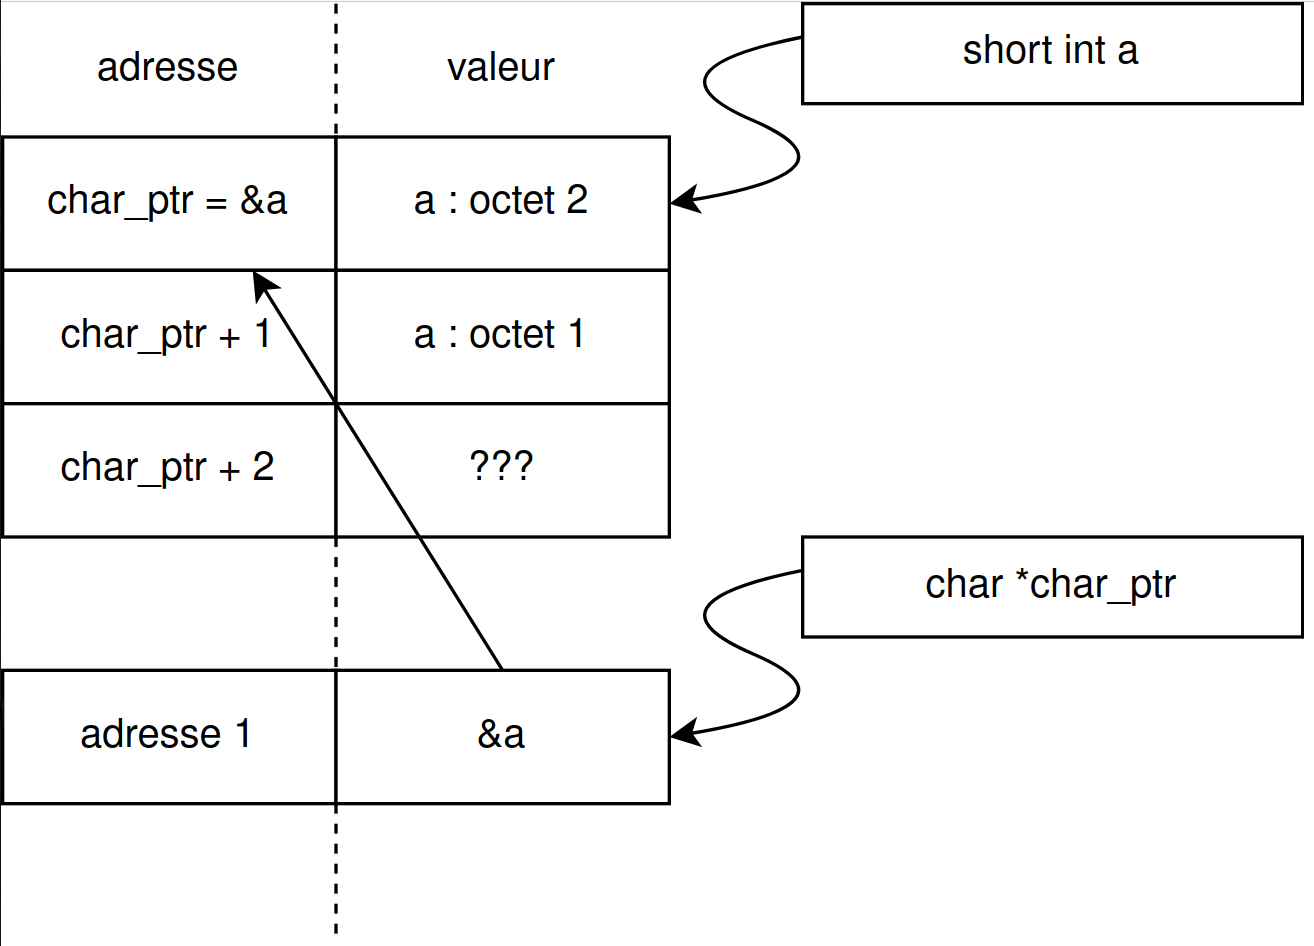
\includegraphics[width=\textwidth]{pointeur3}
	\end{center}
\end{minipage}
 
Ainsi, toutes les égalités du code suivant sont vraies :
\begin{minted}[linenos=false]{c}
char *char_ptr = char_ptr;
short int *sint_ptr = char_ptr;
int *int_ptr = char_ptr;
long int *lint_ptr = char_ptr;

// tous les tests d'égalité suivants sont vrais :
char_ptr == sint_ptr;
char_ptr == int_ptr;
char_ptr == lint_ptr;
char_ptr + 4 ==	int_ptr + 1;
char_ptr + 2 == sint_ptr + 1;
sint_ptr + 2 == int_ptr + 1;
int_ptr + 2 == lint_ptr + 1;
\end{minted}
Et de manière plus générale pour tout \textsf{TYPE} et pour tout $n$ :
\begin{minted}[linenos=false]{c}
TYPE* ptr = char_ptr;
ptr + n == char_ptr + sizeof(TYPE) * n
\end{minted}
Toutefois, un détail reste troublant\dots l'inversion des octets 1 et 2 sur le schéma ci-dessus, que l'on observe à l'exécution du programme sur n'importe quel ordinateur possédant un UCC \textit{Intel}. 
Aucune reformulation ici, l'explication sur Wikipédia suffit : \url{https://fr.wikipedia.org/wiki/Boutisme}\footnote{Ce document n'est pas un cours d'histoire de l'informatique :`$|$}.
 
\textbf{Notation :} Avant de partir dans quelques exercices, voyons simplement une facilité d'écriture du langage C, valide pour tout pointeur \textsf{ptr} et tout entier \textsf{i} :
\begin{minted}{c}
// le résultat du test suivant est toujours vrai
ptr[i] == *(ptr + i);
\end{minted}
Plus un petit \textit{trick} inutile mais rigolo : comme l'addition est commutative on peut aussi écrire :
\begin{minted}{c}
// le résultat du test suivant est toujours vrai
(i - 1)[ptr + 1] == *(ptr + i);
\end{minted}
Les raisons de l'existence de cette facilité d'écriture seront détaillées dans la section \ref{sec:tableaux_statiques} sur les tableaux.
\subsubsection{Le pointeur quelconque : \textsf{void*}}
\label{ssub:le_pointeur_quelconque_void_}
Un dernier cas d'utilisation du projecteur de type est celui du pointeur quelconque \textsf{void*}. En soi, un pointeur contient seulement une adresse, et il peut être intéressant dans certains programmes (voir la section \ref{sec:allocation_dynamique} sur les tableaux dynamiques) de ne conserver que l'adresse et d'``oublier'' le reste, c'est-à-dire le type du pointeur.
 
Le type spécial \textsf{void*} représente exactement cela : un pointeur non typé vers une adresse.
 
La projection de type sur un pointeur non typé \textsf{void*} permet de faire retrouver au pointeur un type :
\begin{minted}{c}
void *pointeur_quelconque = NULL;

// projection de type explicite pour éviter les avertissements à la compilation
int *int_ptr = (int*)pointeur_quelconque; 
\end{minted}
Par ailleurs, l'addition sur un pointeur non typé est ``classique'' :
\begin{minted}{c}
void *pointeur_quelconque = NULL;
printf("%p\n", pointeur_quelconque + 5); // -> 0x5
\end{minted}
Si pour l'instant l'utilisation de tels pointeurs peut rester assez absconse, cela s'éclairera dans le chapitre sur les concepts avancés du langage C. On trouvera déjà un premier exemple dans la section \ref{sec:allocation_dynamique} sur les tableaux dynamiques qui montre une application essentielle des pointeurs.
\subsection{Pointeurs itérés}
\label{sub:pointeurs_it_r_s}
\begin{minipage}{\textwidth}
	\begin{center}
		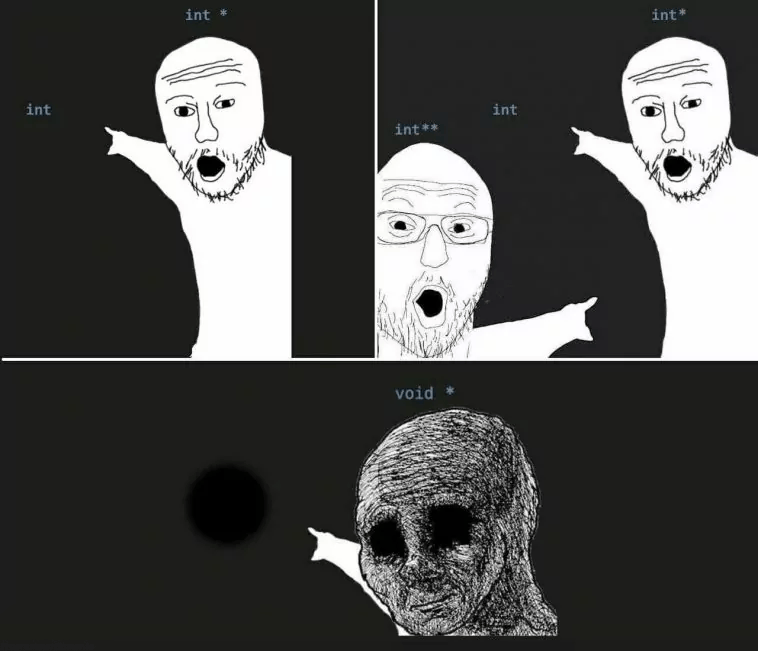
\includegraphics[width=.75\textwidth]{pointer_meme}
	\end{center}
\end{minipage}

On laisse au lecteur le plaisir d'essayer, ce qui lui permettra de se familiariser avec les concepts.
\subsection{Exercices}
\exercise{Quelques procédures inutiles pour devenir un bot efficace}{10} Programmer en C les procédures suivantes, et les tester sur quelques valeurs :
\begin{itemize}
	\item \textsf{void mov(int *x, int val);} : assigne à la variable pointé par $x$ la valeur $val$
	\item \textsf{void add(int *a, int *b);} : assigne à la variable pointée par $a$ la somme des valeurs des variables pointées par $a$ et $b$
	\item \textsf{void mul(int *y, int *z);} : assigne à la variable pointée par $y$ le produit des valeurs des variables pointées par $y$ et $z$
	\item \textsf{void pow(int *x, int n);} : assigne à la variable pointée par $x$ la valeur de la variable pointé par $x$ à la puissance $n$
\end{itemize}
\exercise{Interversion sans effet de bord (3)}{10} Écrire une procédure \textsf{void swap(int *a, int *b);} qui échange les valeurs des variables pointés par $a$ et $b$ sans utiliser de variable temporaire. Quel est le comportement du programme si $x = y$ ? (c'est-à-dire que la même adresse est passé en argument pour les deux paramètres) \newline
Si cela induit une erreur de comportement de la procédure, corriger cette erreur.
 
\exercise{Distance de Manhattan}{25} Cet exercice est là uniquement comme exercice technique\footnote{et rigolo (?)}. La méthode utilisée est à la fois inefficace et immonde à lire et à programmer. On se rapportera aux \textbf{Structures} pour un implantation correcte.
\begin{enumerate}
	\item Écrire une fonction \textsf{double coords\_to\_point(float x, float y);} qui stocke les coordonnées d'un point dans une seule variable de type \textsf{double} à l'aide d'une projection de type.
	\item Écrire une fonction \textsf{double substract(double pA, double pB);} qui à deux points $p_{A} = (x_{A}, y_{A})$ et $p_{B} = (x_{B}, y_{B})$ renvoie : $$p_{A} - p_{B} = (x_{A} - x_{B}, y_{A} - y_{B})$$
	\item Écrire une fonction \textsf{float norme1(double p)} qui calcule la norme 1 d'un point $p = (x, y)$ :
	$$\lVert{\vec{p}}\rVert = |x| + |y|$$
	\item En déduire une fonction \textsf{float distance(double pA, double pB);} qui renvoie la distance entre deux points $p_{A}$ et $p_{B}$ associée à la norme 1. Cette distance est appelée \textit{distance de Manhattan}\footnote{Souvent utilisée en informatique du fait de sa vitesse d'exécution.}
\end{enumerate}
\textbf{Remarque : }On pourra éviter les avertissements à la compilation en effectuant des projections de type explicites.

\exercise{Valeur absolue (2)}{18}En utilisant seulement des projections de type et une opération bits-à-bits, écrire une fonction \textsf{float abs(float x);} qui calcule la valeur absolue de $x$.

\exercise{Racine carrée inverse rapide (2)}{25}
Reprendre le résultat de l'\refexercise{Racine carrée inverse rapide (1)} pour écrire une fonction \textsf{float fast\_inverse\_square\_root(float x);} qui calcule $\frac{1}{\sqrt{x}}$ par une simple transformation linéaire.
\end{document}